\documentclass[conference]{IEEEtran}
% \IEEEoverridecommandlockouts
% The preceding line is only needed to identify funding in the first footnote. If that is unneeded, please comment it out.
%Template version as of 6/27/2024

\usepackage{cite}
\usepackage{amsmath,amssymb,amsfonts}
\usepackage{algorithmic}
\usepackage{graphicx}
\usepackage{textcomp}
\usepackage{xcolor}
\usepackage{booktabs}
\usepackage{url}
\def\BibTeX{{\rm B\kern-.05em{\sc i\kern-.025em b}\kern-.08em
    T\kern-.1667em\lower.7ex\hbox{E}\kern-.125emX}}

% Condition names as in the benchmark output. The prose uses plain names (shared LP, SMT sibling, E-cores,
% baseline, idle-sibling control); the monospace names appear only in the table, the figures, and where Section III
% defines them. Terms: batch latency (wake to batch end); update period (50 ms) and its deadline (the end of the
% period); cost (a placement's change in the game's frame time against its matched control).
\newcommand{\cond}[1]{\texttt{#1}}

\begin{document}

\title{GRU Placement in a Synthetic Game Loop on a Hybrid Laptop CPU}

% The department names are split over two lines so that all three author blocks fit in one row.
\author{
\IEEEauthorblockN{Xavier Gonzalez}
\IEEEauthorblockA{\textit{Dept. of Electrical Engineering}\\
\textit{and Computer Science}\\
\textit{Texas A\&M University--Kingsville}\\
Kingsville, TX, USA\\
xavier.a.gonzalez@students.tamuk.edu}
\and
\IEEEauthorblockN{Haitham Adarbah}
\IEEEauthorblockA{\textit{Dept. of Electrical Engineering}\\
\textit{and Computer Science}\\
\textit{Texas A\&M University--Kingsville}\\
Kingsville, TX, USA\\
Haitham.Adarbah@tamuk.edu}
\and
\IEEEauthorblockN{Jesus Guillen}
\IEEEauthorblockA{\textit{College of Computing}\\
\textit{Georgia Institute of Technology}\\
Atlanta, GA, USA\\
jguillen6@gatech.edu}
}

\maketitle

\begin{abstract}
On hybrid laptop processors, neural-network inference for enemy artificial intelligence (AI) can interfere with the latency-sensitive game thread. This work places one gated recurrent unit (GRU) inference thread on the game thread's logical processor (LP), on its Performance-core simultaneous multithreading (SMT) sibling, or on the Efficient-cores (E-cores) of an Intel Core i9-12900H running a calibrated synthetic game loop at its thermal limit. Across 180 configurations, 3,240 block-randomized tests compared each placement with a matched no-AI control. The median increase in mean frame time was 0.12~ms on the E-cores, 1.60~ms on the SMT sibling against an idle-sibling control, and 6.10~ms on the shared LP; because the controls differ in background work, these are marginal costs, not an equal-work ranking. E-core mean batch latency was a median of 1.83 times that on the SMT sibling of the busy game core. At a 50-ms update period, 104 configurations on the E-cores, 129 on the SMT sibling, and none on the shared LP had no observed missed deadline in three trials. A validation session reproduced these results. With the same background work in all three placements, the E-cores gave the lowest mean frame time in every block, a median of 9.86~ms against 12.30~ms on the SMT sibling and 13.85~ms on the shared LP. Without pinning, Windows started 99.9\% of the AI thread's batches on the E-cores, at a cost within 0.02~ms of manual E-core placement. The results hold for one synthetic workload on one laptop.
\end{abstract}

\begin{IEEEkeywords}
hybrid processors, P-cores, E-cores, simultaneous multithreading, gated recurrent units, game AI, inference latency, thread placement
\end{IEEEkeywords}

\section{Introduction}
Neural networks have been applied to non-player-character behavior, including learned navigation agents evaluated in a AAA game engine \cite{alonso}. Recurrent networks can predict the future positions of moving agents \cite{alahi}, and the gated recurrent unit (GRU) is simpler to compute than the long short-term memory unit \cite{cho}. When such inference runs on the central processing unit (CPU), it competes with rendering, physics, and other engine work, and a game targeting 60 frames/s has 16.67~ms to produce each frame.

Intel's 12th-generation (Alder Lake) laptop processors turn this competition into a placement decision. They combine Performance-cores (P-cores), each running two hardware threads through simultaneous multithreading (SMT), with single-threaded Efficient-cores (E-cores) \cite{rotem2022}. Enemy-AI inference can therefore share the game thread's own logical processor (LP), run on the other hardware thread of the game's P-core (its SMT sibling), or run on the E-cores. This paper compares these placements against matched no-AI controls. Its contribution is a measured tradeoff among marginal frame-time interference, batch latency, and deadline success in a synthetic game loop, not a new scheduling policy.

\section{Background and Related Work}
Intel's game-development guide names AI and pathfinding as candidates for the E-cores and describes a scheduling goal of using SMT siblings last to avoid contention \cite{gerasimov}. Yet the two hardware threads of a P-core share its execution resources \cite{tullsen} and slow each other by amounts that depend on what each executes \cite{snavely}. The P-cores and E-cores also share the last-level cache \cite{gerasimov}, and all cores share the package power budget \cite{rotem2012}, which software can observe through the running average power limit (RAPL) interface \cite{khan}.

If AI decisions update asynchronously, inference need not finish inside a frame, but it must meet its own update period without delaying the game thread. In a user study, average frame rate alone predicted player quality of experience poorly, whereas the bottom 5\% of frame rates appeared to predict it well \cite{liu}; this paper uses the 99th-percentile frame time, which that study did not test.

On Alder Lake, an evaluation on Linux found limitations in the per-thread hints of Intel Thread Director \cite{saez2022}. Recent work balances large language model (LLM) inference across the unequal cores of Intel hybrid CPUs \cite{luo2024} or adapts CPU--GPU inference to changing hardware load on consumer machines \cite{atsinfer}. Closest to this study, Chen et al. found that GPU-only LLM inference beside a mobile game on a Snapdragon 8 Gen 3 dropped its frame rate to zero during prefill, whereas splitting the work between the GPU and the neural processing unit did not \cite{chen2025}. No study identified in this review has measured, against matched controls, both a game's frame-time cost and the latency of periodic inference on each CPU placement of a hybrid laptop processor.

\section{Experimental Method}
\subsection{Platform and Placement Conditions}
The experiment ran on an MSI Pulse GL66 12UEK laptop with an Intel Core i9-12900H processor (6 P-cores with 12 LPs, 8 E-cores, and a 24-MiB last-level cache) and 32~GB of DDR4-3200 memory, under Windows 11 Pro 25H2 (build 26200.9457) with virtualization-based security and hypervisor-enforced code integrity on. The laptop ran on AC power with no graphics load. MSI Center's Extreme Performance mode set the configured package power limits (PL1 and PL2) to 200~W, above Intel's 115-W maximum turbo power \cite{intelspec}, so cooling rather than a power limit set clock speeds. Windows used its Best performance power mode on the Balanced scheme. Airplane mode was on, and nonessential applications and services were stopped.

% Power settings as logged. OEM mode: MSI Center Extreme Performance (operator notes; HWiNFO PL1 = PL2 = 200 W).
% Windows: Best performance power mode (overlay ded574b5-45a0-4f42-8737-46345c09c238) on the Balanced scheme
% (381b4222-f694-41f0-9685-ff5bb260df2e), the only scheme installed for the main and control sessions (run_metadata.txt and
% run_benchmark_log.txt); run_validation.bat switched to it and checked the overlay for the validation session.

Five conditions differed only in where the AI thread ran and whether the worker thread on LP~1 was parked (blocked, using no CPU time; Fig.~\ref{fig:placement}). The game thread always ran on LP~0, and worker threads on LP~1 to LP~11 ran the game workload continuously, standing in for the rest of a game's CPU load. The shared-LP placement (\cond{P\_SHARED}) pinned the AI thread to LP~0. The SMT-sibling placement (\cond{P\_SMT}) parked the worker on LP~1, the sibling of LP~0, and pinned the AI thread there. The E-core placement (\cond{E\_CORE}) allowed its single AI thread on LP~12 to LP~18 and left the choice to Windows. The baseline (\cond{BASELINE}) ran no AI and was the matched control for the shared-LP and E-core placements; the idle-sibling control (\cond{SMT\_IDLE}) parked the LP~1 worker without adding the AI and was the matched control for the SMT-sibling placement. The telemetry and main threads ran on LP~19. The harness read back every affinity mask it set, stopping on a mismatch; where the AI thread actually ran was recorded only in the validation session.

\begin{figure}[t]
\centering
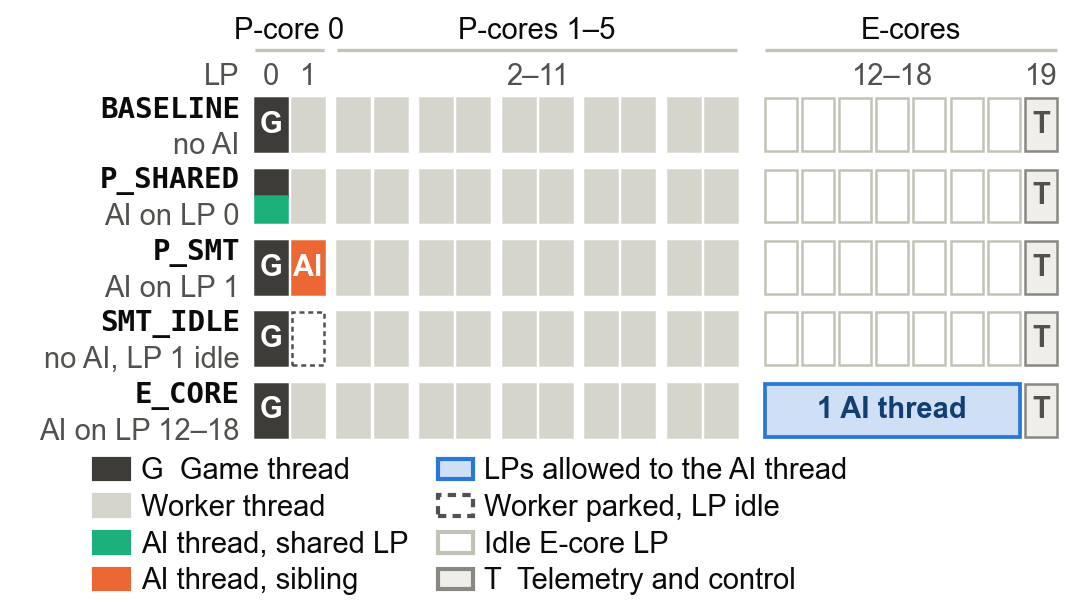
\includegraphics[width=\columnwidth]{figures/fig1_placement.png}
\caption{Thread placement in the five conditions. Rows are conditions and columns the LPs of the Core i9-12900H; LP~0 and LP~1 are the two hardware threads of P-core~0.}
\label{fig:placement}
\end{figure}

\subsection{Models and Benchmark Harness}
Each model is a PyTorch 2.7.1 GRU, exported with ONNX 1.19.1 at opset 17, with a fully connected head on its last step, briefly trained (two epochs) on 500 synthetic 10-step trajectories to predict the next three-dimensional position. The short training creates executable graphs, not accurate navigation models: for fixed dense float32 operators and runtime settings, inference time depends on a model's shape, not on its trained weight values. Outside the timed path, an output-verification mode of the harness ran every model and agent count on the benchmark inputs and three random inputs with the timed settings; all 720 outputs were finite, repeatable, bitwise identical on a P-core and an E-core LP, and within $1.5\times10^{-5}$ of a float64 PyTorch reference, comparable to PyTorch's own float32 error of up to $1.7\times10^{-5}$. Input widths $\{10,100,1000\}$, hidden widths $\{32,64,128,256,512\}$, and layer counts $\{1,2,4,8\}$ give 60 models, each run at 50, 100, and 200 agents, for 180 configurations. Counting a multiply--add as two operations and only dense matrix products, not biases, gate nonlinearities, or runtime overhead, the approximate work of one batch in million floating-point operations (MFLOP) is
\begin{equation}
W=\frac{A}{10^{6}}\left[10\left(6H(I+H)+12H^{2}(L-1)\right)+6H\right],
\label{eq:work}
\end{equation}
where $A$ is the agent count, $I$ the input width, $H$ the hidden width, and $L$ the layer count; $W$ ranged from 4.0 to 53,331~MFLOP; the grid spans batches far shorter and far longer than one update period and models no particular game.

The C++ harness, built with MSVC 19.39 (C++20, /O2), ran all threads at the same base priority in a high-priority process with Windows power throttling disabled. The game workload, a synthetic trigonometric loop over a 1.5-MiB buffer, was calibrated after a 180-s soak under full worker load to a median of 16.0~ms on LP~0. Each test applied the condition's worker set, ran a 60-frame drift check, started the game and AI threads, warmed up the model with six batches, and measured at least 1,000 game frames and 50 batches. A drift-check median more than 15\% from its reference (16.0~ms, or 9.47~ms with the LP~1 worker parked) flagged the test. ONNX Runtime 1.27.1 used its default CPU execution provider in float32 with all graph optimizations and one intra-operation thread, the calling thread, in sequential mode \cite{ortthreading}, so all inference ran on the AI thread itself. All agents formed one batch on fixed synthetic inputs in a tensor created once, with a zero initial hidden state; the timer enclosed one ONNX Runtime call and the sum of its outputs. One batch was scheduled per 50-ms update period on an absolute clock, and the end of each period was that batch's deadline. A batch that ended after its deadline missed it; the next batch then started at once and the periods restarted from that point, so skipped periods were neither queued nor counted. Each completed batch counts as one update, and miss rates divide misses by updates; a batch still running when the window closed was discarded.

\subsection{Design and Metrics}
Each configuration and trial formed a block whose conditions ran back to back in random order, and the 540 blocks were shuffled with a fixed seed. The main session ran the baseline and the three placements in 2,160 tests over 12~h. The idle-sibling control was added afterward, and a control session the next night ran it and the SMT-sibling placement in the same blocks and order with the same calibration (1,080 tests).

The harness recorded the mean and nearest-rank 99th-percentile (P99) frame time, the mean and P99 batch latency, missed deadlines, and the duty cycle, the share of the window spent inside batches. Batch latency runs from when the AI thread woke to when its batch ended, whereas the deadline is fixed at the end of the update period, so a batch with low latency could still miss its deadline by starting late; this start delay, which with batch latency makes up the release-to-completion time, was recorded only in the validation session. The results therefore report both P99 batch latency within the update period and deadline success, a configuration with no observed missed deadline in its three trials. Each placement is compared with its matched control in the same block as an absolute difference and as a relative change, $(x_{\mathrm{placement}}/x_{\mathrm{control}}-1)\times100\%$, and a placement's change in the game's frame time is its cost: the marginal interference against its own no-AI workload. Because the SMT-sibling placement parks a worker, whose lost work the harness did not measure, the costs do not rank total frame time for equal work. Package power came from the RAPL energy meter \cite{khan} and processor performance from the Windows \% Processor Performance counter, both about every 110~ms; because the counter is a frequency-based percentage averaged over the P-core LPs, not a per-core clock, it is compared only between conditions with the same busy LPs. HWiNFO64 logged package temperature, clocks, and limit flags every 2~s. Reported changes are medians of the 540 paired changes with 95\% percentile bootstrap confidence intervals (CIs). Because the three trials of a configuration are not independent, the bootstrap resamples the 180 configurations, each with all three trials, 2,000 times, and two-sided Wilcoxon signed-rank tests use the 180 configuration medians \cite{wilcoxon}. The medians summarize the tested grid, not a population of models.

A validation session 18 days later used the same calibration to run 16 configurations spanning the work range and deadline boundaries in three trials (432 tests). Besides the five conditions, it ran the E-core and shared-LP placements with the LP~1 worker parked, giving all three placements the same work, and, against the baseline, an unpinned AI thread and one pinned to LP~12 alone. The harness also traced each frame and each batch's scheduled and actual start, end, LPs, and thread cycles. Measurement windows lasted at least 20~s, and effects use their first 20~s, 400 update periods in every condition; comparisons with earlier sessions use the window the original stopping rule would have produced, and CIs resample the 16 configurations. The harness, scripts, configuration lists, and raw data are available at \url{https://github.com/xavie-Codes/CoresResearch}.

\section{Results}
\label{sec:results}
% Every number in this section comes from the outputs of audit_analysis.py and doc_tables.py (paper_files/tables):
% effects_summary, deadlines, drift_order, replication, impact (Fig. 2), ai_latency and throughput (Fig. 3),
% ecore_dose and ecore_weights (E-core subsection), psmt_duty, shared_stall, control_hwinfo, hwinfo_refresh, facts and
% paper_facts, absolute (measured frame times, updates per test), architecture (architecture-level bootstrap and
% tests), and doc/ai_summary, doc/operating_point, doc/doc_facts and doc/effect_tests. The C++ output check in
% Section III-B: cpp_output_check.csv (verify_cpp_outputs.py on the harness's --verify-outputs folders). The validation
% session (Sections III-C and IV-F, and its numbers in IV-D and IV-E): validation_analysis.py (paper_files/tables/validation),
% mainly facts.csv, with replication, deadlines, same_work, residence, timing, effects_equal20 and hwinfo.
\subsection{Data Quality and Operating Point}
\label{sec:quality}
All 3,240 tests, and the 432 validation tests, completed without drift flags or truncated windows, and each configuration's output checksum was the same in every placement, trial, and session. One retained E-core test increased the game's mean frame time by 30.5\% while the AI was busy only 9\% of the time; the next-largest E-core cost was 2.4\%, and the medians are insensitive to this outlier.

Drift stayed below the flag threshold, with the baseline's mean frame time rising 0.20~ms (1.2\%) over the 12-h main session, and each placement's cost kept its sign and approximate size whether it ran before or after its control.

The sessions ran at the thermal limit, although sampling cannot confirm this for every test: the package averaged 94.7~\textdegree C at about 45~W in each session, and its thermal-throttling flag was set in 99.9\% to 100\% of HWiNFO samples, although that of P-core~0 never was; no power-limit, PROCHOT, or current-limit flag was set. P-core~0 ran at a median of 3.09 to 3.19~GHz per session against a 5.0-GHz turbo ceiling \cite{intelspec}. HWiNFO's per-core sensors and package power refreshed only every 80 to 110~s (median) in the main session but every 2~s in the control and validation sessions.

\subsection{Game-Thread Cost}
E-core placement cost a median of 0.12~ms of mean frame time (Table~\ref{tab:effects}), against 1.60~ms for the SMT sibling (relative to the idle-sibling control) and 6.10~ms for the shared LP, and the P99 frame-time costs were 0.05, 3.91, and 28.3~ms (all $p<0.001$). Resampling the 60 architectures instead of the 180 configurations widened the mean-cost intervals to [0.09, 0.15], [0.87, 2.94], and [3.61, 13.77]~ms, still with $p<0.001$ on the architecture medians. In measured frame time, the SMT-sibling placement was fastest because its worker was parked; at equal work, the E-cores were (Section~\ref{sec:validation}). Its median P99 frame time, 17.38~ms, exceeded the 16.67-ms frame budget.

The cost grew with the AI's work at very different rates (Fig.~\ref{fig:gamecost}). Below 100~MFLOP per batch, every placement's median cost stayed at or below about 6\%. Above 3,000~MFLOP, where the AI thread was busy at least 98\% of the time, the cost leveled off near $+100\%$ on the shared LP and near $+90\%$ on the SMT sibling, and the shared LP's P99 cost reached 359\%. The E-cores' median cost stayed below 1.3\% in every bin.

% Source: audit_analysis.py. Placement / control rows: absolute.csv. Change rows, the configuration-level Wilcoxon
% tests, and the batch-latency ratios: effects_summary.csv. Configuration and deadline counts and missed deadlines:
% deadlines.csv.
\begin{table*}[t]
\caption{Game and AI Costs of Each Placement Against Its Matched Control}
\label{tab:effects}
\centering
\footnotesize
\begin{tabular}{@{}lccc@{}}
\toprule
Measure & \cond{E\_CORE} vs.\ \cond{BASELINE} & \cond{P\_SMT} vs.\ \cond{SMT\_IDLE} & \cond{P\_SHARED} vs.\ \cond{BASELINE} \\
\midrule
\multicolumn{4}{@{}l}{\textit{Game and package (paired blocks; \cond{P\_SMT} from the control session)}} \\
Mean frame time, placement / control, ms & 16.25 / 16.12 & 11.32 / 9.69 & 22.20 / 16.12 \\
P99 frame time, placement / control, ms & 16.53 / 16.48 & 17.38 / 13.20 & 44.74 / 16.48 \\
Mean frame time change, ms & $+0.12$ [0.10, 0.14] & $+1.60$ [1.11, 2.41] & $+6.10$ [4.43, 10.36] \\
P99 frame time change, ms & $+0.05$ [0.04, 0.07] & $+3.91$ [2.80, 4.67] & $+28.3$ [23.2, 41.1] \\
Package power change, W & $+1.48$ [1.19, 1.69] & $+1.26$ [1.08, 1.54] & $+0.49$ [0.38, 0.56] \\
\midrule
\multicolumn{4}{@{}l}{\textit{AI (all three placements from the main session)}} \\
Configurations with P99 batch latency $\le$ 50~ms & 108 of 180 & 129 of 180 & 76 of 180 \\
Configurations with no observed missed deadline in three trials & 104 of 180 & 129 of 180 & 0 of 180 \\
Mean batch latency relative to \cond{P\_SMT}, median & 1.83 & 1.00 & 1.87 \\
Tests with at least one missed deadline & 41.1\% & 28.3\% & 99.4\% \\
\bottomrule
\end{tabular}
\\[4pt]
\parbox{\textwidth}{\footnotesize Placement / control rows are medians over the 540 tests of each condition, measured directly. Change rows are medians of 540 paired changes against the matched control, with 95\% cluster-bootstrap CIs over the 180 configurations in brackets; Wilcoxon signed-rank tests on the configuration medians gave $p<0.001$ for every change in frame time and package power. Configurations are counted by their median P99 over three trials. Shared-LP batch latency includes waits for the game thread during a batch but not before it.}
\end{table*}

\begin{figure*}[t]
\centering
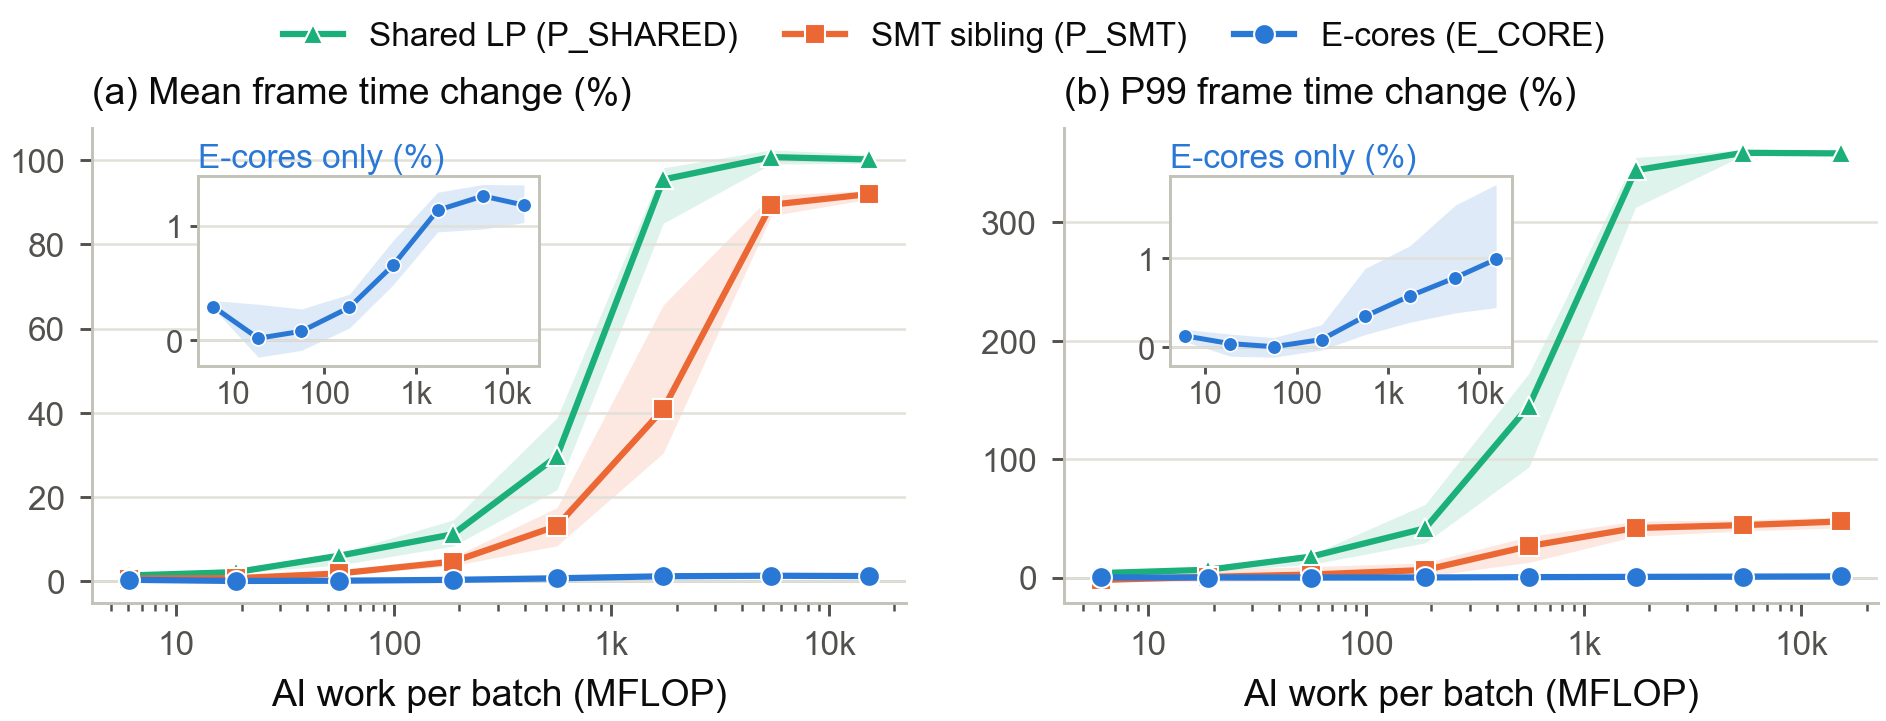
\includegraphics[width=0.75\textwidth]{figures/fig2_game_cost.png}
\caption{Game frame-time cost versus AI work per batch: (a) mean and (b) P99 frame time change against the matched control. Points are medians over the blocks in each bin of work (edges at 10, 30, 100, 300, 1,000, 3,000, and 10,000~MFLOP; 6 to 120 blocks per bin); bands show the interquartile range, and insets repeat the E-core series on its own scale.}
\label{fig:gamecost}
\end{figure*}

\subsection{Inference Latency and Deadlines}
On the E-cores, P99 batch latency fit the 50-ms update period for every configuration up to 1,358~MFLOP per batch except one at 1,333~MFLOP, and for none above, so 108 of the 180 fit (Fig.~\ref{fig:ailatency}a). On the SMT sibling, the same held up to 2,716~MFLOP except at 2,667~MFLOP (129 fit). These crossings are observations, not capacity limits: in each pair, with $H=256$ and $L=2$, the member with $I=1000$ and half the agents had the lower P99, so shape, not work alone, set the latency. On the shared LP, every configuration below 188~MFLOP fit, none above 802~MFLOP did, and 76 fit in all. E-core mean batch latency was 1.35 to 2.06 times that on the SMT sibling of the busy game core, not intrinsic core-speed ratios; the gap widened with hidden width, from 13.5 against 19.6 billion floating-point operations per second (GFLOP/s) at $H=32$ to 30.6 against 62.5~GFLOP/s at $H=512$ (Fig.~\ref{fig:ailatency}b).

P99 batch latency within the update period did not guarantee deadline success. On the E-cores, 104 of the 108 configurations that fit had no observed missed deadline in three trials; the other four, with P99 batch latencies of 44.0 to 49.3~ms, missed at most 1.8\% of deadlines, in tests that also had batch latencies above 50~ms, so every configuration below 44~ms (88\% of the period) met every deadline. All 129 configurations that fit on the SMT sibling met every deadline, although over a median of 635 updates in three trials, against 972 on the E-cores. No shared-LP configuration met every deadline: 99.4\% of shared-LP tests missed at least one, including 176 tests in which every batch latency was under 50~ms, because the AI thread started late while the game thread held LP~0 (Section~\ref{sec:mech}).

\begin{figure*}[t]
\centering
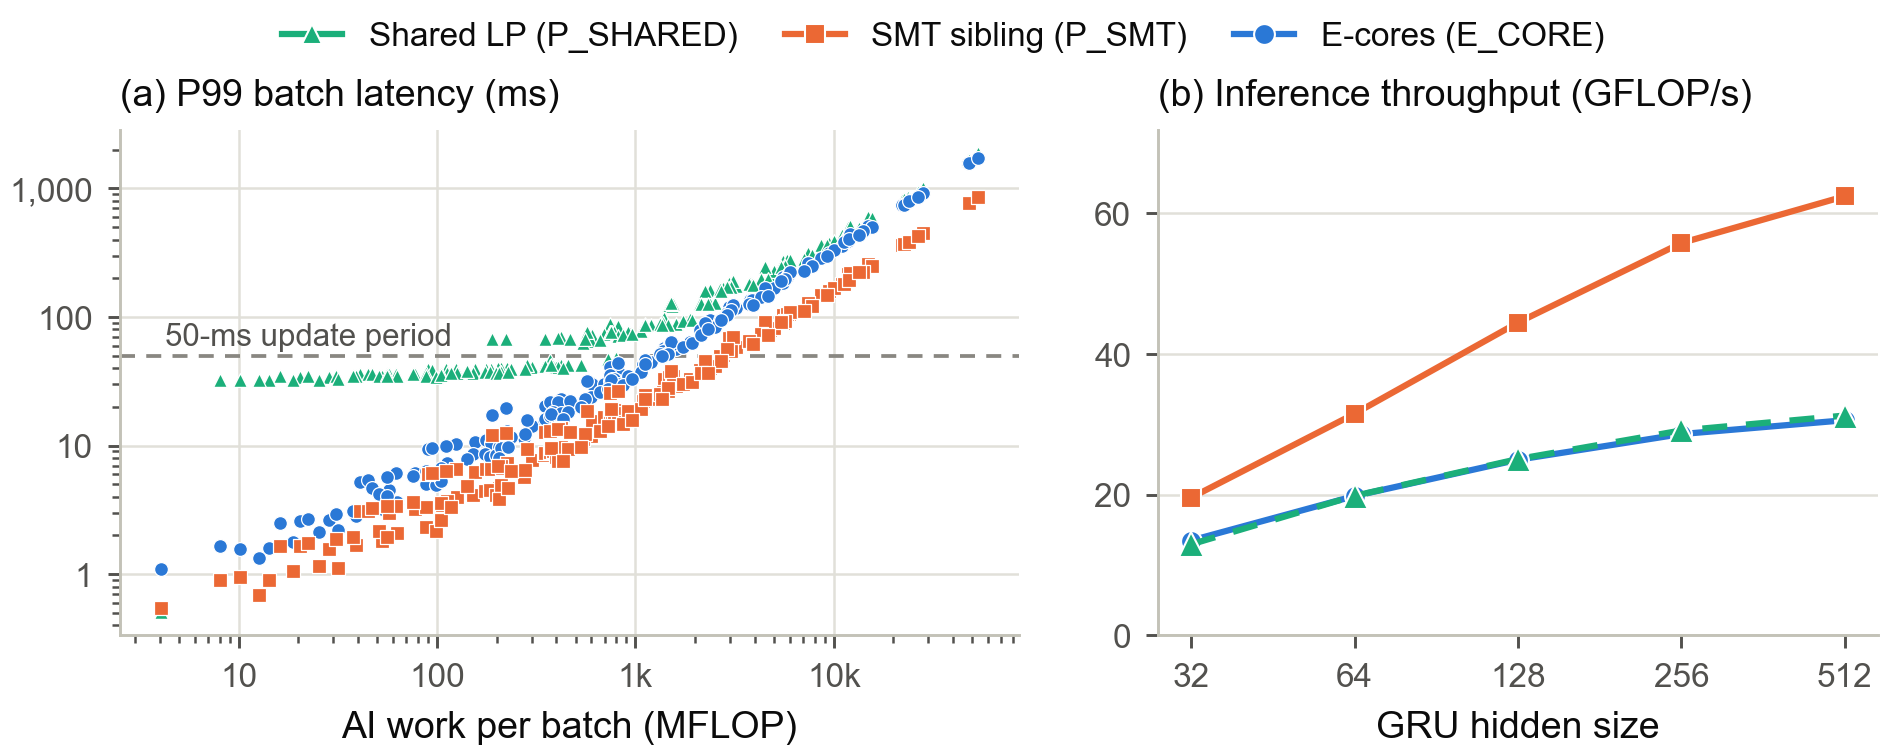
\includegraphics[width=0.75\textwidth]{figures/fig3_ai_latency.png}
\caption{AI batch latency and throughput by placement: (a) P99 batch latency of each configuration and placement (median of three trials, main session), with the 50-ms update period dashed; configurations below it could still miss deadlines. (b) Median inference throughput, work per batch divided by mean batch latency, by hidden width. The 216 tests with fewer than 100 batches, all above 4,400~MFLOP, have the maximum as their nearest-rank P99.}
\label{fig:ailatency}
\end{figure*}

\subsection{E-Core Offload and the Shared Thermal Budget}
As the E-core AI's duty cycle rose from under 10\% to 100\%, the median change in package power rose from $+0.16$ to $+2.40$~W, the change in P-core \% Processor Performance fell from $-0.08$ to $-1.15$ points, and the cost rose from $+0.07\%$ to $+1.16\%$ of mean frame time. At the thermal limit, added E-core power would be offset by lower P-core clock speeds: a 1.15-point drop from the baseline level of about 109 is about 1.1\%, close to the cost, and in the validation session, P-core~0's clock was 22~MHz (0.7\%) lower during E-core tests than in the baseline, 95\% CI [11, 33]~MHz, against a 0.9\% cost there. Cache and memory contention would grow with the model's weights, yet when the E-core AI never idled, the median cost stayed at 1.14\% to 1.20\% in weight groups spanning 1.3 to 51.0~MiB, beyond the 24-MiB last-level cache. The observations are thus consistent with thermal coupling, but cache, memory, and other shared-resource effects were not isolated: no cache-miss or bandwidth counters were collected.

% The duty-cycle figure (figures/fig4_ecore_thermal.png) is left out to meet the six-page limit; the numbers it plots
% are in the paragraph above. To restore it, uncomment the block below and add (Fig.~\ref{fig:thermal}) after the
% first sentence of this subsection.
% \begin{figure*}[t]
% \centering
% 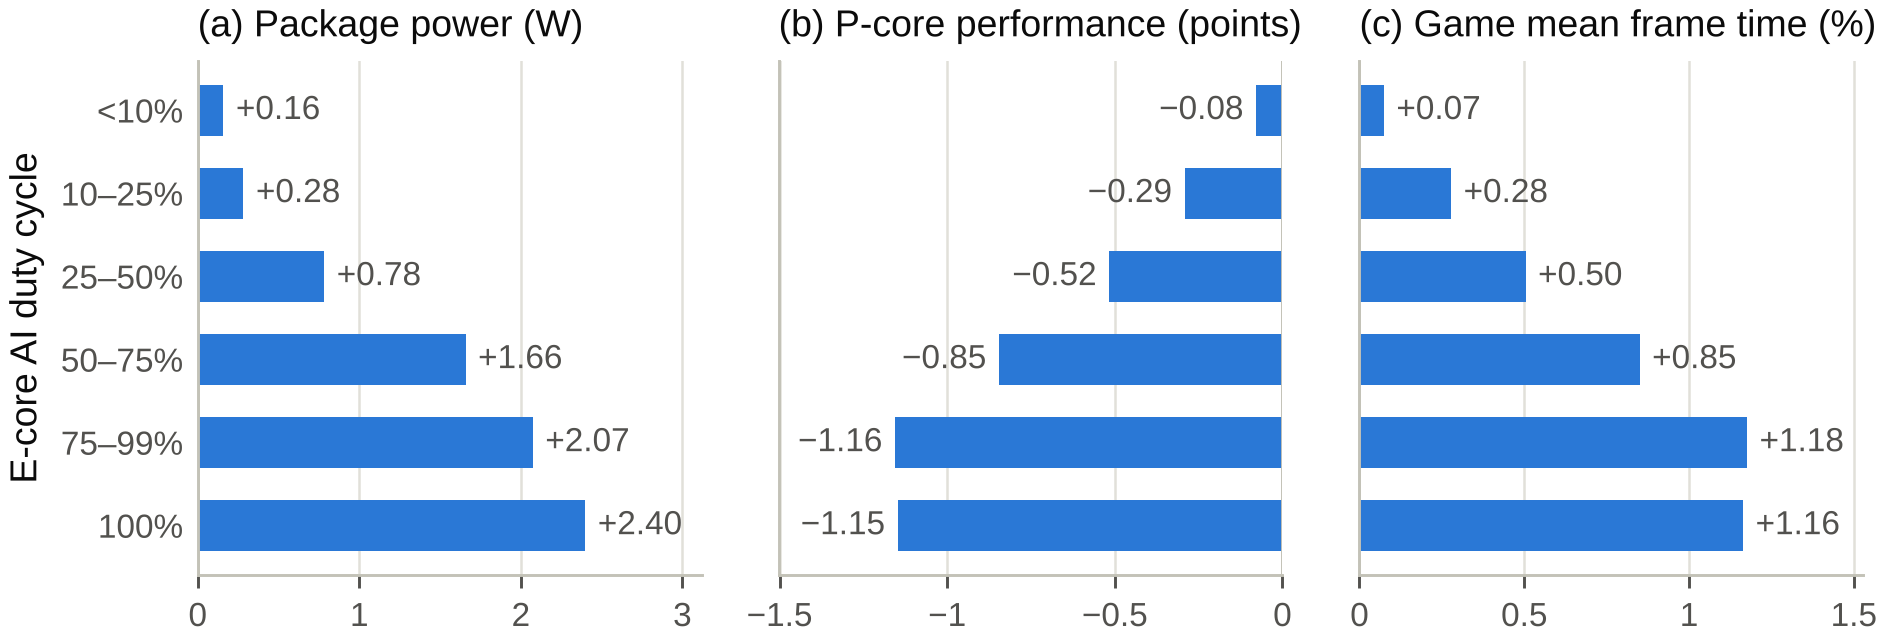
\includegraphics[width=0.8\textwidth]{figures/fig4_ecore_thermal.png}
% \caption{Cost of E-core offload at the thermal limit by E-core AI duty cycle: (a) package power, (b) P-core \% Processor Performance, and (c) game mean frame time, as medians of the changes against \cond{BASELINE} of the same block (89, 88, 75, 51, 33, and 204 blocks, lowest band first).}
% \label{fig:thermal}
% \end{figure*}

\subsection{Mechanisms of the P-Core Placements}
\label{sec:mech}
Against the idle-sibling control, the SMT sibling's cost grew with the AI's duty cycle on LP~1, from $+0.6\%$ below 2\% duty to $+90.6\%$ when the AI never idled, while HWiNFO recorded the same P-core~0 clock, 3,180~MHz, in SMT-sibling and idle-sibling tests, so the evidence points to sharing the core, not a lower clock, as the cause.

On the shared LP, when the AI never idled, the game's mean frame time was 32.3~ms against 16.15~ms in the baseline, so the game received about half of LP~0. This pattern is consistent with Windows running equal-priority threads on one LP in turns of one time slice \cite{mssched}: a batch shorter than a time slice tends to run to completion while the game waits, whereas a longer batch is preempted when its slice ends. The validation traces show both: shared-LP batches below 100~MFLOP started a median of 13.9~ms after their scheduled start (P99 31.7~ms), which caused 41 of their 42 missed deadlines, yet were on the CPU for a median of 99.9\% of their batch latency, whereas batches of at least 1,000~MFLOP were on it for only 68\%.

\subsection{Validation Session}
\label{sec:validation}
Over the original rule's windows, each configuration's validation mean and P99 frame times were within 3.0\% and 6.6\% of their earlier values in every condition. The median costs of the E-cores, SMT sibling, and shared LP were 0.15, 2.52, and 10.78~ms, against 0.17, 2.41, and 10.42~ms for the same configurations, and the same configurations as before fit within 50~ms and met every deadline on the E-cores (11 and 7) and on the SMT sibling (14 and 14), counts that equal 20-s windows left unchanged. With the LP~1 worker parked in all three placements, the E-cores gave the lowest mean frame time in every block, a median of 9.86~ms against 12.30~ms on the SMT sibling and 13.85~ms on the shared LP. Left unpinned, the AI thread started 99.9\% of its batches on an E-core LP, and its cost matched the E-core placement's within 0.02~ms. The E-core AI thread used all seven allowed LPs and started 53\% of its batches on a different LP than the previous one ended on; pinned to LP~12 alone, it cost the same but had a 1.4-ms higher P99 batch latency and 17\% more missed deadlines. E-core and SMT-sibling batches started within 0.69 and 0.53~ms of their scheduled start in 99\% of cases, and 96\% of E-core misses were batches longer than 50~ms.

\section{Discussion}
\subsection{Placement Guidelines}
The E-cores cost the game about 1\% even at saturation and gave the lowest frame time at equal work, supporting Intel's guidance \cite{gerasimov}; the cost is consistent with coupling through the shared thermal budget, which a rule based only on shared execution resources would miss. Three guidelines follow for a game whose main thread occupies a P-core; with every other P-core LP busy, Windows itself placed an unpinned AI thread on the E-cores. First, run neural enemy AI on the E-cores, allowing all of them rather than one LP, when its measured release-to-completion time, at the miss rate the game tolerates, leaves a margin within the update period; here, no E-core configuration with a P99 batch latency below 88\% of the period missed a deadline. Second, use the SMT sibling only for light models and only when it would otherwise be idle: below 300~MFLOP per batch, its median cost was 0.25~ms (2.6\%) of mean frame time. Third, avoid sharing the game thread's LP, where scheduler delays affected both threads and even light models missed deadlines.

\subsection{Threats to Validity}
The results come from one laptop at one cooling-limited operating point, with every other P-core thread loaded and no graphics load. Other processors, coolers, and power-limited states may change the costs and latency ratios. In a game, the graphics processor would also heat the same chassis, so the thermal limit would likely bind harder.

The shared-LP costs depend on the Windows time slice, which varies by system \cite{msmultitask} and was not recorded, and on priority boosts \cite{msboost}, which the harness left enabled; a game normally owns the foreground window, unlike this high-priority console program, so these magnitudes may not transfer. Time slicing was inferred from start delays and thread cycles, not traced.

The game workload is a synthetic loop calibrated in duration, without an engine's instruction mix, synchronization, rendering, or graphics load; the models received brief training on synthetic trajectories and were not validated for navigation accuracy; and inference used one thread with all agents batched.

The idle-sibling control was added after the main session, and the validation session repeated only 16 configurations. The drift check ran only before each window, so disturbances during a window, such as the E-core outlier in Section~\ref{sec:quality}, were not flagged. Room temperature and the MSI Center Cooler Boost setting were recorded only for the validation session (25.6~\textdegree C, off), and fan speeds not at all.

\section{Conclusion}
In the tested synthetic game loop at the thermal limit, E-core placement produced the smallest marginal frame-time increase and, at equal background work, the lowest frame time, and Windows chose the E-cores for an unpinned AI thread; the SMT sibling completed inference faster and had more configurations without observed missed deadlines. Sharing the game thread's LP produced substantial interference and missed deadlines even for light models. Deployment decisions should use absolute frame times, release-to-completion time, and an acceptable deadline-miss rate under the intended engine workload. These measurements set no universal MFLOP threshold and do not isolate thermal coupling as the cause of the E-core cost.

\section*{Acknowledgment}
Claude (Anthropic), used through Claude Code, helped revise the benchmark program, launchers, and training script before the main session, later added the idle-sibling control, output verification, and the validation conditions and traces without changing how frame time or batch latency was measured, wrote the analysis and figure scripts, and drafted text for the authors' review. The authors take full responsibility for the content.

% References are numbered in order of first citation. Each entry was checked against its source for the claim it
% supports; entries without pages or a DOI could not be verified to that level of detail.
\begin{thebibliography}{00}
\bibitem{alonso} E. Alonso, M. Peter, D. Goumard, and J. Romoff, ``Deep reinforcement learning for navigation in AAA video games,'' in \textit{Proc. 30th Int. Joint Conf. Artif. Intell. (IJCAI)}, 2021, pp. 2133--2139, doi: 10.24963/ijcai.2021/294.
\bibitem{alahi} A. Alahi, K. Goel, V. Ramanathan, A. Robicquet, L. Fei-Fei, and S. Savarese, ``Social LSTM: Human trajectory prediction in crowded spaces,'' in \textit{Proc. IEEE Conf. Comput. Vis. Pattern Recognit. (CVPR)}, 2016, pp. 961--971, doi: 10.1109/CVPR.2016.110.
\bibitem{cho} K. Cho, B. van Merri\"{e}nboer, C. Gulcehre, D. Bahdanau, F. Bougares, H. Schwenk, and Y. Bengio, ``Learning phrase representations using RNN encoder--decoder for statistical machine translation,'' in \textit{Proc. Conf. Empirical Methods Natural Lang. Process. (EMNLP)}, 2014, pp. 1724--1734, doi: 10.3115/v1/D14-1179.
\bibitem{rotem2022} E. Rotem \textit{et al.}, ``Intel Alder Lake CPU architectures,'' \textit{IEEE Micro}, vol. 42, no. 3, pp. 13--19, May 2022, doi: 10.1109/MM.2022.3164338.
\bibitem{gerasimov} P. Gerasimov, M. du Bois, and L. Davies. ``Game dev guide for 12th Gen Intel Core processor.'' Intel Corporation, Jun. 13, 2022. Accessed: Oct. 28, 2026. [Online]. Available: \url{https://www.intel.com/content/www/us/en/developer/articles/guide/12th-gen-intel-core-processor-gamedev-guide.html}
\bibitem{tullsen} D. M. Tullsen, S. J. Eggers, and H. M. Levy, ``Simultaneous multithreading: Maximizing on-chip parallelism,'' in \textit{Proc. 22nd Annu. Int. Symp. Comput. Archit. (ISCA)}, 1995, pp. 392--403, doi: 10.1145/223982.224449.
\bibitem{snavely} A. Snavely and D. M. Tullsen, ``Symbiotic jobscheduling for a simultaneous multithreaded processor,'' in \textit{Proc. 9th Int. Conf. Archit. Support Program. Lang. Oper. Syst. (ASPLOS)}, 2000, pp. 234--244, doi: 10.1145/378993.379244.
\bibitem{rotem2012} E. Rotem, A. Naveh, A. Ananthakrishnan, E. Weissmann, and D. Rajwan, ``Power-management architecture of the Intel microarchitecture code-named Sandy Bridge,'' \textit{IEEE Micro}, vol. 32, no. 2, pp. 20--27, Mar. 2012, doi: 10.1109/MM.2012.12.
\bibitem{khan} K. N. Khan, M. Hirki, T. Niemi, J. K. Nurminen, and Z. Ou, ``RAPL in action: Experiences in using RAPL for power measurements,'' \textit{ACM Trans. Model. Perform. Eval. Comput. Syst.}, vol. 3, no. 2, Art. no. 9, pp. 1--26, Jun. 2018, doi: 10.1145/3177754.
\bibitem{liu} S. Liu, A. Kuwahara, J. J. Scovell, and M. Claypool, ``The effects of frame rate variation on game player quality of experience,'' in \textit{Proc. CHI Conf. Human Factors Comput. Syst.}, 2023, Art. no. 573, pp. 1--10, doi: 10.1145/3544548.3580665.
\bibitem{saez2022} J. C. S\'{a}ez and M. Prieto-Mat\'{\i}as, ``Evaluation of the Intel Thread Director technology on an Alder Lake processor,'' in \textit{Proc. 13th ACM SIGOPS Asia-Pacific Workshop Syst. (APSys)}, 2022, pp. 61--67, doi: 10.1145/3546591.3547532.
\bibitem{luo2024} Y. Luo, Y. Liu, and H. Shen, ``A dynamic parallel method for performance optimization on hybrid CPUs,'' 2024, arXiv:2411.19542.
\bibitem{atsinfer} Y. Liu, H. Ye, M. Li, and W.-J. Li, ``Automated tensor scheduling for hybrid CPU-GPU LLM inference on consumer devices,'' 2026, arXiv:2607.10183.
\bibitem{chen2025} L. Chen \textit{et al.}, ``Characterizing mobile SoC for accelerating heterogeneous LLM inference,'' in \textit{Proc. ACM SIGOPS Symp. Oper. Syst. Princ. (SOSP)}, 2025, pp. 359--374, doi: 10.1145/3731569.3764808.
\bibitem{intelspec} Intel Corporation. ``Intel Core i9-12900H processor (24M cache, up to 5.00 GHz) specifications.'' Accessed: Oct. 28, 2026. [Online]. Available: \url{https://www.intel.com/content/www/us/en/products/sku/132214/intel-core-i912900h-processor-24m-cache-up-to-5-00-ghz/specifications.html}
\bibitem{ortthreading} ONNX Runtime Project. ``Thread management.'' Accessed: Oct. 28, 2026. [Online]. Available: \url{https://onnxruntime.ai/docs/performance/tune-performance/threading.html}
\bibitem{wilcoxon} F. Wilcoxon, ``Individual comparisons by ranking methods,'' \textit{Biometrics Bull.}, vol. 1, no. 6, pp. 80--83, Dec. 1945, doi: 10.2307/3001968.
\bibitem{mssched} Microsoft. ``Scheduling priorities.'' Microsoft Learn. Accessed: Oct. 28, 2026. [Online]. Available: \url{https://learn.microsoft.com/en-us/windows/win32/procthread/scheduling-priorities}
\bibitem{msmultitask} Microsoft. ``Multitasking.'' Microsoft Learn. Accessed: Oct. 28, 2026. [Online]. Available: \url{https://learn.microsoft.com/en-us/windows/win32/procthread/multitasking}
\bibitem{msboost} Microsoft. ``Priority boosts.'' Microsoft Learn. Accessed: Oct. 28, 2026. [Online]. Available: \url{https://learn.microsoft.com/en-us/windows/win32/procthread/priority-boosts}
\end{thebibliography}

\end{document}
